\chapter{緒論}

% 標題: (近紅外光)任兩點 LED與光電二極體 室內 任兩點 三維相對位置 最佳化組態

\section{前言} %(工業4.0的篇幅)

隨著工業4.0的發展,機器、人與環境之間的交互互動愈發頻繁,藉由物聯網(IoT)的能力,各領域對於量測資訊的需求大量增加,其中物聯網所包含的應用領域包含智慧工廠、智慧病房、智慧城市等如圖\ref{pic:iot}\cite{iot}。

\begin{figure}[ht]
    \centering
    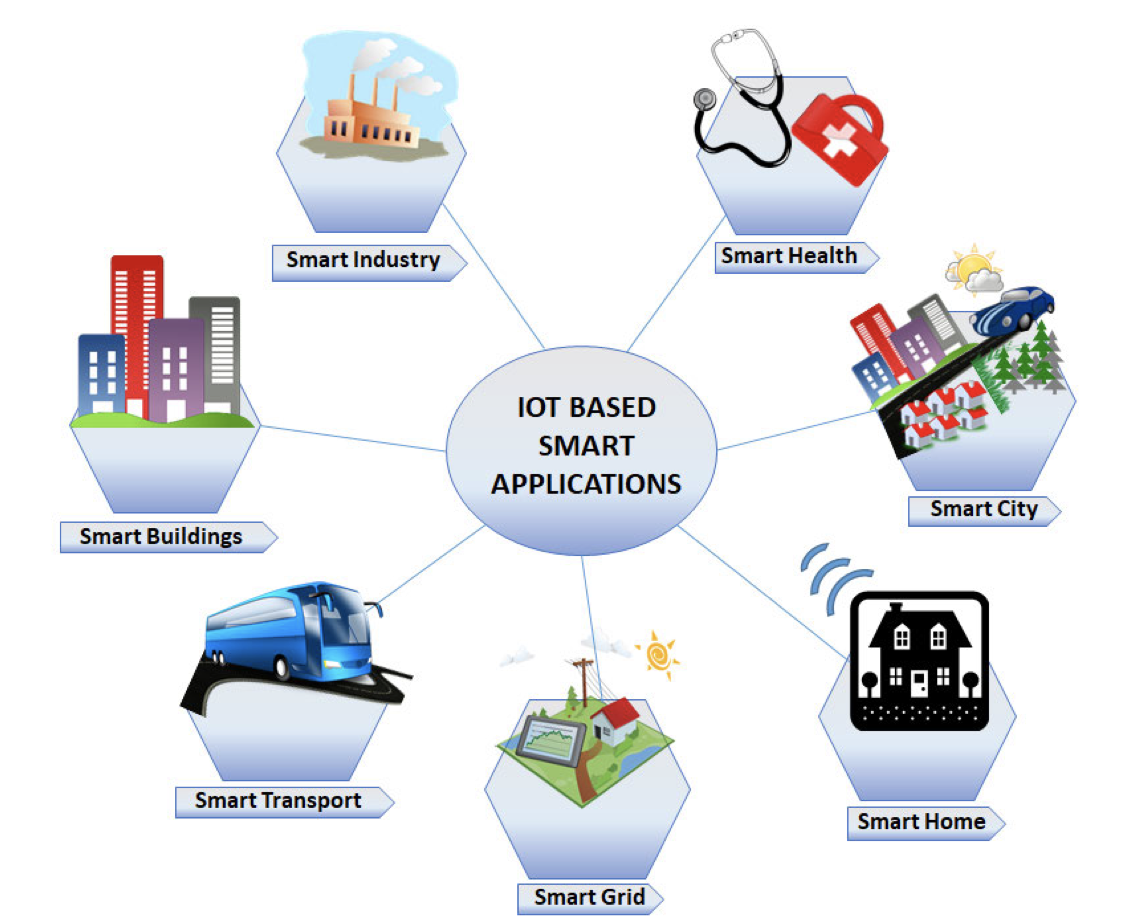
\includegraphics[width=10cm]{ch1pic/iot.png}
    \caption{物聯網應用的領域\cite{iot}}
    \label{pic:iot}
\end{figure}

在萬物互連的背景之下,感測器就像是人類的感官,透過不同種類的感測器量測各式各樣所需的資訊,例如位置、溫度、濕度、電壓、電流、轉速、流速、振動、影像等,各物體之間交換資訊,再透過電腦或是人為操作,下達任務與決策。各項量測資訊之中相對位置實為重要,缺乏位置資訊的狀況就像是失去地圖的駕駛或是被蒙住眼睛的人們,無論是移動、導航、指令的下達與否的各種重要決策與行為都會難以判斷。然而,定位在實務上充滿挑戰,由於沒有任何一種感測器可以直接量測到相對位置,僅能透過多個感測器量測到的距離、角度、影像等資訊進行校正與運算以獲得定位資訊,並不像是量測距離、溫度等感測器得以直接獲得的物理量一樣簡單。



室外場域中,相對位置需求最常見於載具,例如無人機之間的相互定位,以及自駕車之間的跟隨與溝通;除了載具以外,相對定位的量測在搜救、目標跟隨、監視等情況下都有需求\cite{outdoor_scenario}。現今室外定位主要仰賴全球衛星定位系統(Global Positioning System,以下簡稱GPS)\cite{GPS_important},其透過接收三個以上的衛星訊號,由各訊號傳輸時間判斷與各衛星的距離,進而獲得接收者的位置。即使現今的GPS既容易取得又有相對高的精度\cite{survey_light2020},礙於衛星訊號受建築物體遮蔽的特性,GPS仍然無法在市區、室內等障礙物較多的場域取得有效的定位\cite{survey_light2018},


室內定位主要面對的困難與室外不同,室內定位需面對較多的障礙物、牆壁、人員物體的密集度,這些障礙物使多重路徑傳輸(Multipath propagation)影響大,也使訊號衰減與散射較為嚴重,以上議題都會增加誤差與難度。眾多文獻都提到相較室外定位,室內定位的難度更高\cite{survey_light2020}\cite{survey_light2018}\cite{survey_indoor2014}\cite{survey_indoor2018}\cite{survey:indoor_wayfinding},且使用的硬體與演算法百百種,各方法的優缺點也不同,因此至今仍沒有一個領先群雄的方法。為了從眾多室內定位方法中挑選合適者,我們於\ref{chp:motivate}章釐清本研究的目標使用情境,再於\ref{chp:intro}章了解室內定位需考量的面向,以便挑選出最合適的系統。






\section{研究動機}
\label{chp:motivate}
% 前言

本論文所針對的目標情境如圖\ref{pic:imagine},以兩個可攜式單位進行定位,當兩單位於空間中自由移動時,其中一單位可量測到與另一單位之間的三維相對定位。然而,現今大多系統皆是針對特定場域與地點、需大量事先校正與設置,但凡更換環境該系統則失效,難以廣泛應用。因此,我們的主要目標是為了提供一彈性拆裝、能夠廣泛應用的設計,以彌補現今定位系統缺少的靈活度。

\begin{figure}[ht]
    \centering
    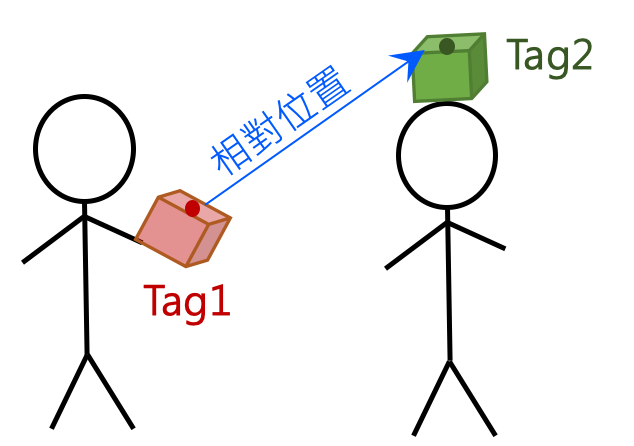
\includegraphics[width=7cm]{ch1pic/imagine.png}
    \caption{本論文所針對的目標情境}
    \label{pic:imagine}
\end{figure}

為了達到以上情境,我們希望系統有以下的特點:

\begin{enumerate}
    \item 感測器與訊號發射器可包裝成可攜式的單位,因此需選擇大小適中、能耗低的硬體。
    \item 兩量測單位皆需有易安裝、易移動的特性,得以靈活的將兩單位各自安裝在量測物與目標物上。
    \item 能夠在不同環境與場域中進行三維的相對定位量測。
    \item 定位為兩單位之間的定位,不得使用多個參考點。
\end{enumerate}


\hfill

我們認為若能達到上述目標,在應用上將具有很大潛力,以下舉實例描述以更具體呈現:
\begin{description}
    \item[- 智慧工廠] \hfill 
    
    \quad \quad 
    隨著工業4.0與5.0的發展,人機互動以其機器間的互動越加頻繁,且工廠內也會從同品項大量製造,變成變化度高的製程,因此擁有靈活的量測單位實為重要,可以隨時安裝在需定位的人、機械手臂、載具等上面,根據工作不同改變。

    \item[- 智慧病房] \hfill 
    
    \qquad
    隨著輔具、病床智慧化,擁有靈活安裝的定位系統,能夠幫助機器與患者之間的定位,即使患者移動或是醫療器具更換。也能夠重新安裝不受影響。
    
    \item[- 其他]  \hfill 
    
    \qquad
    智能載具與服務目標的定位、輔助視障者理解目標方向、機場內針對各種載具與行李運送的量測、展場內的偵測引導等。
\end{description}

% 補實例圖








\subsection{室內定位考量的面向}
\label{chp:intro}
% 室內定位的簡介:(範圍對點、點對點、應用情境)




室內定位的方法非常多樣化,本論文參考\cite{survey_indoor2018},將室內定位依照硬體的技術(Technology)與後處理的方法(Technique)分類:硬體技術所針對的是目標與量測者傳送訊號所使用的硬體種類,常見的技術包含相機、紅外線、可見光定位、無線網路(以下簡稱WiFi)、藍芽、無線射頻辨識(Radio Frequency IDentification,以下簡稱RFID)等不同技術,於\ref{chp:technique}章中會更詳盡的介紹。

而方法則是探討不同訊號接收與處理的方式,從接收訊號資訊的種類可分為訊號強度、時間、與角度;如何利用所接收到的資訊,進一步解出相對位置則於定位演算法分類,常見的包含多點定位(Multilateration)、三角測量(Triangulation)、指紋法(Fingerprinting)、以及利用幾何關係求解的演算法,於\ref{chp:method}章中會進一步介紹。


在選擇合適的技術與方法以設計室內定位系統時,需考量許多面向,以下介紹室內定位需考量的因素,以及各因素與不同硬體技術(詳述於\ref{chp:technique}章)、後處理方法(詳述於\ref{chp:method}章)的關聯:

\begin{description}
    \item[1. 精度]\hfill 
    
    \qquad
    量測精度為量測所得的位置與目標物真實位置之間的歐幾里德距離(Euclidean Distance,以下簡稱歐式距離),多以公尺表示\cite{survey:indoor_wayfinding},普遍精度最高的技術為相機、紅外光\cite{survey_indoor2014},精度大多會在公分量級上下;相較精度較低的則為WiFi與藍芽,精度常會在公尺量級上下\cite{survey_indoor2014}。然而為了達到高精度,需要與大多面向做取捨\cite{survey:indoor_wayfinding},例如欲達到較高的量測範圍、降低成本、提高靈活度等,都需要捨棄部分精度,難以同時兼顧。
    
    \item[2. 量測範圍] \hfill  
    
    \qquad
    光波段的相機、紅外光、可見光量測範圍大多會限制在五米內,超出此範圍後定位精度會快速下降;而WiFi、藍芽、RFID等覆蓋範圍則較廣,能夠達到十米以上的定位\cite{survey_indoor2014}。
    
    \item[3. 成本] \hfill 
    
    \qquad
    系統成本包含硬體設備成本與系統能耗等,成本與使用的硬體技術種類相關,硬體成本屬於中高價位的有相機、紅外線、RFID,而WiFi、藍芽、可見光定位則屬於建設成本較低的選項;能耗的部分則每篇論文皆有不同的看法,如\cite{survey:radio}中認為WiFi為低能耗相較\cite{survey:indoor_wayfinding}認為其為高能耗,各篇論文中並沒有共識。
    
    \item[4. 環境或是單點對單點的定位] \hfill 
    
    \qquad
    常見的系統架構包含兩種,第一種需在環境中的多個位置放置接收器或是發射器作為參考點,透過建立多個參考點收發訊號來進行定位分析,此種類型的系統固定於環境中,呈現「環境對單點」的定位;另一種為兩個硬體單位之間的定位,呈現「單點對單點」的定位。這邊指的「單點」並不是限制硬體數量,而是指量測次系統與目標物次系統的硬體架設大小,若量測者與目標物兩個硬體單位,皆能封裝成兩可移動單位,則屬於單點對單點的定位;而兩者主要取決於方法中的演算法類型。

    \qquad
    舉例來說,後處理方法中的指紋法需在空間中建立多個參考點,事先蒐集大量數據建立數據庫,定位時再利用數據庫中的資料做交叉比對,此方法便屬於環境對單點的定位,需花大量時間事先校正,且不能適應環境的改變,但凡環境與系統異動則原數據庫失效,大大限制了應用靈活度。環境對單點的定位中,系統大多能透過提高參考點的數量來提升精度與量測範圍。眾多硬體技術中,訊號精度較低的硬體技術如WiFi、藍芽、RFID較侷限在這種大規模的系統,應用靈活度低。反之,相機使用的視覺辨識方法,大多是利用單個相機擷取目標物的影像,透過辨識目標物的形狀等來判斷定位,無論是相機單位還是目標物單位都是一個個體,屬於單點對單點的定位。

    


    
    \item[5. 是否定位可視範圍外] \hfill 
    
    \qquad
    非可視範圍(Non-Line-of-Sight,以下簡稱NLoS)的定位,會擴大量測範圍,即可不受到環境障礙物的影響,即便是隔著牆壁也可以進行定位。然而此舉也同時會造成訊號來源混亂,無法分辨此訊號強度為LoS傳遞而來的,還是穿透何種障礙物之後造成衰減的訊號,進而犧牲精度。而能夠穿透障礙物的多屬於使用低頻率電磁波的硬體技術,如WiFi、藍芽、RFID,此特性也反應較低的精度上。


    \item[6. 即時應用性] \hfill 
    
    \qquad
    需進行即時應用的情境下,量測數據處理速度需夠快,以避免訊號延遲,因此經常犧牲訊號處理的複雜度及其附加的精度,或是提高成本增加硬體運算能力。訊號處理複雜度高最容易聯想到的便是相機,為了進行視覺辨識的高運算,該類型的系統多配備較好的演算單位\cite{survey_light2020};除此之外,主要影響因素則是該系統的演算法速度,各項技術與方法皆有演算法快與慢的方法,如何設計便是精度、功能豐富度與運算速度之間的取捨。
    
    \item[7. 目標物是否為特定物] \hfill 
    
    \qquad
    定位技術大多指目標物為特定某物體的情況,因此系統需有分辨訊號發送者的能力,例如WiFi、藍芽、RFID都具有傳送訊息的能力且發展成熟\cite{survey:indoor_wayfinding},可見光與紅外線則是利用近年發展的光通訊方法進行訊號傳輸,而相機則是利用視覺辨識判斷目標物;反之,超聲波與光達僅有分辨訊號的有無,難以進行目標物辨識,因此大多應用在判斷障礙物存在與否的情境,較少在定位系統上出現。
    
    \item[8. 場域限制]\hfill 
    
    \qquad
    特別需要注意的是機場與醫院,這兩種場域有可能會限制無線電波的使用\cite{case:vlc_mobile},因此使用無線電波段的技術如WiFi、藍芽、RFID則需特別注意。
\end{description}

\hfill

礙於以上如此多的特性與面向,一個面面俱到的方案是不存在的。因此在設計系統時,了解不同做法的優缺點,並了解系統目標情境與需求,進而對不同面向做出取捨,是完成有效室內定位系統的關鍵之一\cite{survey_indoor2018}。












%[看最後能不能凹到一開始發想是在醫療器具上,結合實驗室研究,這樣可見光就變更合理了]

\section{研究目的}
\label{chp:purpose}

根據\ref{chp:motivate}章中提到的使用情境,我們的目標是建立一系統,其中觀察者與目標物皆可封裝為兩硬體單位,具有可攜式、易於安裝的特性,以達到單點對單點的定位。因此,在\ref{chp:intro}章中提出的多個面向,我們需著重在4.中的單點對單點的定位,希望硬體系統可封裝成兩單位,以及3.成本中的低能耗特性。

雖然室內定位這個領域已經有許多文獻探討,然而針對單點對單點的定位與低能耗這兩個特性,仍待一個更合適的方案。因此以這幾個面向為重點,於\ref{chp:method}章與\ref{chp:technique}章中逐漸聚焦於發光二極體(Light Emitting Diode,以下簡稱LED)與光電二極體(Photodiode,以下簡稱PD)的近紅外光定位。針對此種硬體技術,設計一不限制應用場域,且目標物能夠自由移動的定位演算法,主要改善現今定位系統的侷限度,並將LED與PD定位系統中經常被忽略的硬體參數以及組態完整加入考慮。除了提出演算法外,本研究有會進行模擬與分析,並針對不同使用情境進行最佳化,透過挑選合適的硬體參數與組態,以提升系統定位成效。

% 以下以條列呈現本論文的研究目的:

% \begin{itemize} 
%     \item{探討現今定位技術與方法}:為了發展一靈活度高,能夠套用在不同場域與情境的室內定位方法,探討不同硬體技術與後處理方法的特性,將研究聚焦在LED與PD定位上。
%     \item {深入了解LED與PD定位}:LED與PD定位的理論開始介紹,接著介紹現行LED與PD定位方法,由此呈現此領域所不足的地方:光波段定位的領域中,為了降低系統的複雜度,經常限制使用情境,例如限制目標物與觀察者需為平行。
%     \item{提出廣用於演算法}:因此本論文提出一不需限制情境的三維定位演算法,且將常被文獻忽略的朗博次方與硬體指向同樣納入考量。
%     \item{完整模擬}:建立一軟體模擬環境,模擬LED與PD定位系統,並
%     \item{針對情境最佳化}:將提出的演算法套用在不同的使用情境上,發展一套完整流程,針對其進行組態與硬體參數的最佳化。
% \end{itemize}

% 補想像圖








\section{論文架構}
本研究分為六個章節,論文架構如下:

\begin{description}
    \item[第一章] 緒論
    
    \qquad 介紹研究主題,並描述本研究欲解決的問題與研究目的。
    
    \item[第二章] 室內定位相關文獻探討
    
    \qquad 
    介紹室內定位的不同硬體技術與後處理方法,並聚焦在利用LED與PD的光定位方法,介紹此領域現行方法與現今研究所不足之面向。
    
    \item[第三章] 建立廣用於三維空間的LED與PD定位演算法
    
    \qquad 
    為改善現今文獻中演算法不足處,建立一利用LED與PD的三維相對定位演算法,此演算法不需限制接收與發射平面平行,且將常被文獻忽略的朗博次方與硬體指向同樣納入考量。

    \item[第四章] 模擬與評估系統表現
    
    \qquad 
    建立一模擬系統,以第三章所提出的演算法進行模擬定位流程,並提出量化系統定位成效的方法,並透過分別調整不同次系統設計參數與誤差來分析各參數對系統成效影響。
    
    \item[第五章] 針對不同使用情境進行次系統最佳化
    
    \qquad 
    針對不同的使用情境,將次系統設計作為變數,進行系統成效的最佳化。
    
    \item[第六章] 結論
    
    \qquad 
    整理本研究之結果討論,並敘述後續研究之方向。
    
    \end{description}







    %